\documentclass{IEEEtran}
\usepackage{graphicx}
\usepackage{color}
\usepackage{setspace}
\usepackage{multirow}
\usepackage{rotating}
\usepackage{flushend}
\usepackage{multicol}


\begin{document}

\title{Secure Local Data Aggregation and Delay Tolerant Dissemination in VANETs}
\author{\IEEEauthorblockN{Cesar Ghali \quad\quad Sky Faber \quad\quad
Kyle Benson \quad\quad Quan Nguyen}\\
\IEEEauthorblockA{Group Number 1, Computer Science Department\\
University of California, Irvine \\
$\{$\texttt{cghali, fabers, kebenson, quann1}$\}$@uci.edu}
}
\maketitle

\begin{abstract}

Recent advances in wireless networking and sensing technologies have brought about research trends in enabling vehicles to communicate with each other while driving.  These vehicular ad-hoc networks (VANETs) could automate the vehicles themselves and/or greatly decrease dangers inherent with driving by warning each other of hazards and reacting to them.
Due to the limited bandwidth and connectivity of wireless mediums and the large quantities of data being generated in such a system, novel techniques must be explored for aggregating and disseminating useful information so that it can be made available in a reliable and timely manner.
In this paper, we propose a method of securely, quickly, and locally disseminating aggregate information about crash events and other hazards in VANETs.
We show our technique's efficacy through simulation in NS-3 \cite{ns3}.
\end{abstract}

\section{Introduction}

Our problem of interest is distributed event detection in wireless sensor networks. Specifically, we are interested in detecting vehicle crash events in vehicular ad hoc networks (VANETs).
When a vehicle is in any kind of collision it will affect both nearby vehicles and vehicles that may be rapidly approaching the crash site.
Therefore, warning these other vehicles about such an event could enable them to take immediate evasive actions to mitigate the possibility of another crash.
Each vehicle that witnesses the crash, as well as the one(s) involved in it, should each take part in notifying others so that as much detail about the nature of the event and possible affects can be cataloged as possible.
Because many vehicles may be present during such an event, they may flood the wireless channel with information if it is not properly aggregated and disseminated to possibly affected entities.

We developed a protocol in which nodes broadcast aggregated packets to nearby nodes in order to forward them along to parts of the network that haven't yet been notified.
This quickly disseminates data about the event occurrence to vehicles that may be affected by the collision, whether from extra traffic congestion or possible road hazards/debris.
At the same time, messages from different participants that witnessed the crash are aggregated together into a single packet, while still preserving information about which nodes detected the crash.
This decreases overall bandwidth consumption while still delivering the same information about crash witnesses and potential dangers.
By exploiting mobility patterns of VANETs, our protocol quickly covers nearby nodes with this information in a variety of traffic conditions, as will be shown in the discussion about simulation results.

As an additional consideration, security also becomes an important issue in this scenario.
Detection of an event may have real world repercussions, such as causing vehicles to reroute or completely stop and so our protocol must ensure that no attacker can fake a crash event in order to cause such a reaction.
We briefly catalog known attacks of this type and discuss possible protections against them as well as how our protocol takes them into consideration.

The remainder of the paper is structured as follows.  The second section discusses related works in data aggregation and dissemination.
In the third section, we discuss our protocol in detail.  We present our simulation environment and results from the tests on it in the fourth section.
In the final section, we conclude with a discussion about applications and future work.

\section{Related Work}

In this section, we present several works related to ours in the domains of data aggregation and dissemination.  Much of it is related to wireless sensor networks but can be extended for use in VANETs.

\subsection{Data Aggregation}

In the domain of wireless sensor networks, much recent research has focused on developing aggregation schemes to minimize the amount of power consumed by radio transmissions in order to extend the life expectancy of power-constrained devices that typically rely on batteries.
Many approaches focus on minimum spanning trees (MST) or similar structures because this will require the minimum amount of total power across the whole network.
As shown in \cite{heuristic}, this is because the power required to transmit a radio message is directly proportional with the distance between the nodes.
If sensor nodes can decrease the power of their radios to reach the next hop with minimal energy spent, the MST will give the optimal aggregation of data.

In addition to decreasing energy consumption, these approaches can also be used to reduce communication overhead, thereby freeing up bandwidth for other important messages.
This becomes particularly important in VANETs where the vehicles are envisioned as constantly communicating detailed information with each other.
Here, we discuss aggregation techniques applied to two possible topologies: static and dynamic (mobile nodes).  The latter is likened to VANETs.

\subsubsection{Static Topologies}

In \cite{heuristic}, the minimum-energy aggregation problem is solved by creating a MST in the network that has constraints on the maximum degree of any one node and the maximum number of hops from any node to the sink.  The degree and hop bounds are in place because too high of a degree would put too much load on an individual node and too many hops would require too long for the information to reach the sink.  As the determination of these optimal structures is NP-hard, this paper proposes several heuristics for approximating them.  One of these heuristics, which was determined the best of the proposed three by their simulation results, iteratively builds the MST by adding the next node whose edge has the least weight (power consumption) as long as it doesn’t violate any of the constraints.  If it will, the node is joined to a different parent whose incident edge weight may be higher (thereby making the spanning tree only an approximate MST) but who does satisfy the degree and hop constraints.  If no such parent exists, the parents are recursively checked for the possibility of choosing a new parent for them such that the constraint on the original node can be satisfied.

Another problem which is important in Wireless Sensor Network(WSN) is to schedule the aggregation\cite{DDAS}. The problem is if a node hears two messages at the same time then it can not receive the messages because of message interference. Therefore, in a given graph (V, E), we need to find the schedule which consists of n sets of vertices $S_i$ which satisfies the following properties:
\begin{itemize}
\item $S_i \cap S_j = \emptyset, i \neq j$
\item $\cup_{i=1,n} = V - \{r\}$
\item Data are aggregated from $S_k$ to $V - \cup_{i=1,k}S_i$.
\end{itemize}
To solve this problem, we use the leader election \cite{LeaderElection} algorithm to build the rooted spanning tree. Based on that we will distributed rank each node based on its level(how far from the root) and its identity. Along the computation, we will compute the number of lower-ranked neighbors for each node. Using the computed information, we will build connected dominating set(CDS)\cite{CDS}. Building CDS is the crucial step in different algorithms including the aggregation scheduling problem as it is considered the virtual backbone or spine of wireless ad-hoc network. Finally, we construct the schedule with linear time latency bound on network diameter and maximum node degree.

The above methods consider data aggregation in the network but do not address the issue of time-constrained data transmission.  The authors of \cite{time} address this problem by setting a deadline by which all of the aggregated data should reach the sink.  This deadline is propagated towards the leaf nodes, with each intermediate aggregating node setting its deadline as a function of the number of nodes represented by the aggregated packets it will receive.  Aggregation takes place when either all of the child nodes send their information or the timer expires, thereby ignoring any data not received by this deadline.  This deadline is increased over time but is decreased if the sink does not receive the aggregated messages in time.  In this manner, the timers will converge over time to a point at which the sink’s deadline is respected but the preceding deadlines are late enough to maximize the number of nodes whose data is received by the sink.  The sink must therefore choose a deadline that allows every node in which it is interested to have its data aggregated.  Otherwise, it may misjudge the actual state of the environment being monitored.  Such a scheme is particularly important in time-sensitive applications, such as in VANETs where aggregated information may prevent dangerous crashes.

\subsubsection{Dynamic Topologies}

Some previous works build structures similar to MSTs but focus more on the ability of wireless sensors to broadcast data across an entire region, which may change as the network topology evolves.  A common approach is to cluster nodes and elect leaders for these clusters so that each of the nodes can send their data to the leader, which will then aggregate these packets and send them towards the sink.  This allows a subset of the nodes to transmit messages at longer ranges so that the other nodes can conserve power.  Some such methods also allow for non-static topologies in which nodes may move, join, or leave the network.

The authors of \cite{sct} use the above approach to propose a system that allows for changing the aggregation node so as to distribute the burden of increased power consumption that comes from holding this role as well as tolerate mobile nodes.  The network is broken into a number of concentric rings and sectors within those rings based on the density and size of the network.  Nodes within each sector transfer their data to the node closest to the center of this sector so it can be aggregated and transferred to the next inner ring. The aggregated messages continue to be further aggregated and forwarded, eventually reaching the inner-most ring where they are received by the sink. By varying the locations of these sectors and rings, different aggregation nodes can be chosen and mobile nodes can be followed so as to maintain a balanced number of nodes within each sector.  This balance is particularly important in mobile networks as changing node densities could cause issues of scalability in a static structure.

While the previously mentioned data aggregation methods build a structure over which communication is carried out, \cite{flow} takes an unstructured approach. Here a technique deemed “Flow Updating” is used to perform both broadcast- or gossip-based aggregation without the need of a spanning tree. Here aggregation functions are calculated by exploiting the symmetry of flows in the network. Flows in this context represent portions of the total aggregate value, rather than representing the capacity of an edge as in the traditional graph setting. A node’s local calculation is based entirely on its initial state, and the flow entering the node. Nodes can update their flows with one another either by broadcasting to their neighbors, or using random unicast (gossip). The authors show that this converges considerably faster than older structured approaches. The key idea is that as flows are updated throughout the course of the algorithm, because of directional symmetry, the total aggregate value does not change. Furthermore, flow updating messages are idempotent, a new message simply replaces an old flow with the new value. Because of this idempotence, Flow Updating has good convergence properties, even in the event of link failure. Unfortunately, this method still relies on a static topology, and many rounds of updates, and would not work well with mobile nodes. Furthermore, the authors mention little about calculating aggregate functions that are not based on sum.

Authors in \cite{landmark} describe a technique for aggregating and disseminating travel times in VANETs. Their protocol performs hierarchical aggregation based on the distance from the origin of the data, in this case traffic times of a specific route. The intuition is that nodes physically further away from the origin receive coarser versions of the data. As a vehicle approaches the location, finer-detailed information becomes available so that it may plan a specific route. Nodes in the network share information via broadcast, but aggregate timings according to a hierarchy.

They first define a method for specifying routes with different granularity. A map of a physical street or highway is overlaid with “landmarks”; each landmark defines a specific point of interest on the map and is defined (semi-)manually. Landmarks are then organized hierarchically such that each level in the hierarchy has fewer and fewer landmarks. Times are calculated for landmarks close to each other on the same level in the hierarchy. Nodes in the network measure travel times between two landmarks at the lowest level, and broadcast these times to peers they meet in the same vicinity. As the information travels further from the origin, the nodes compute the distances between landmarks closer to the top of the hierarchy.  Nodes receive only as much information as necessary to make accurate routing decisions.

The \cite{landmark} paper defines very similar functionality as required for our problem. However, traffic data is generated more frequently and requires dissemination to virtually all nodes in the network. While we may not have these constraints, we may be able to apply similar techniques. Unfortunately, the authors simulations are done with additional infrastructure placement and does not compare with any other aggregation techniques.

The aggregation technique used in \cite{prob_agg} is based on Flajolet-Martin sketches. In such sketches a set of elements is represented by a string of bits using a hash function as follows:

\begin{itemize}
\item A string of bits is first initialized to zero.
\item Each element of the set is fed into a hash function.
\item The output of the hash corresponds to an index in the bit array which is then set to 1.
\end{itemize}

When two sketches need to be combined, an OR operation is performed. Moreover, a TTL-based sketch can be used to express lifetime for each entry. Each bit is replaced with a positive integer that is initialized from a maximum value and then is decremented every time the sketch is broadcasted until the bit reaches zero. When two such sketches are aggregated, the maximum value of a specific index is taken, indicating the newest observation of that element in the set. The authors used the proposed Flajolet-Martin-based dissemination to survey the empty spots in a parking lot. Several entities are scanning the parking lot and marking the empty spots using the previous algorithm. At the end, all the collected sketches are aggregated. This algorithm can be used in other applications such as aggregating the existence of some event into a small string of bits data structure.

\subsection{Data Dissemination}

In networks where nodes represent agents within a system, nodes must often disseminate pertinent information to interested parties quickly and reliably.  Constraints such as available bandwidth and network connectivity often encumber these goals and so novel approaches must be taken to ensure delivery of accurate data.   Precision and recall are two metrics that should be taken into considerations while designing such a protocol. Precision is defined as the rate of people getting the content they are interested in to the total number of people getting that specific content, while recall denotes the quantity of interested entities that get the disseminated content.  This section focuses on delay-tolerant dissemination and a study of its application to VANETs.

Flash dissemination requires the distribution of data content to a large number of recipients in a very short time. Such a technique should take into consideration the unpredictable topological changes in the network, scalability to serve large network sizes and the ability to adapt to heterogeneity in the network setup. In \cite{crew}, the authors designed an intelligent flash dissemination protocol, CREW, that outperforms its counterpart protocols in different network setups. CREW is a gossip-based dissemination protocol that is fault-tolerant, decentralized, reduces network overhead.

Since gossip-based dissemination protocols lack the ability of good scalability in large network scenarios, CREW designers modify the push content concept into a pull content concept. In the later approach, each node selects a node at random and exchanges with it the list of all the chunk-ids that it needs. Then, the selected node sends a random chunk to the requester node. This approach reduces the number of broadcasts which fits large networks, and eliminates receiving multiple copies of the same chunk from different gossiping nodes.

Delay Tolerant Networks (DTNs) are new network structures composed of different nodes connected in an ad-hoc fashion. Packet delivery in such networks are based on the best effort model. In which, a node broadcasts the packets it receives to all its neighbor hoping that they will eventually be delivered to their destination, even if an intermediate node must wait for a network connection to be established with the next hop.

On the other hand, a data dissemination protocol for DTNs, Habit is proposed in \cite{habit}. It is to build two directed graphs and share them among all the nodes in the DTN network. The first graph is called the regularity graph which models the physical connections among DTN nodes, and the second graph is called the interest graph which models the shared interests between the nodes. All the nodes in the network share their information about other nodes in order to build an approximate vision of the full graphs of the network. When a node has a message or content to disseminate, it consults with the network representation that it has in order to obtain the shortest paths that the content should traverse to all interested node.

Content dissemination in mobile ad-hoc networks (MANETs) is quite different than in static environments described earlier.
Patterns of interspersed network connectivity and mobility can be exploited to facilitate the spread of information.
VANETs are a special case of MANETs in which the nodes are assumed to move in relatively straight lines, at similar speeds, and with another group of nodes usually travelling in the opposite direction very nearby.
These specific characteristics are leveraged in \cite{vanet_dissem} to develop, compare, and contrast different techniques for dissemination of aggregated data in VANETs.

This particular work advocates for forwarding of messages through a broadcast mechanism as opposed to a unicast to a neighbor of the node.  This is because the data about many vehicles within the network that are close to each other is aggregated together so the broadcast storm problem is mitigated by only having a subset of the vehicles disseminate this information throughout the local network.  The authors consider three different schemes for forwarding this information:

\begin{itemize}
\item Forwarding to vehicles moving in the same direction
\item Forwarding to vehicles moving in the opposite direction on the other side of the road
\item A combination of both techniques (forwarding both directions)
\end{itemize}

By simulating a VANET environment,  the authors discovered that the second technique works best for their scenario.  This is because they aggregate exact locations of vehicles on the road, compressing their coordinates in order to fit within a single message.  This results in more information contained within each message and therefore more lossy compression is required.  By exploiting the mobility of the traffic moving in the opposite direction, these messages can be ferried more quickly and so contain less information, thereby requiring less compression.  In actuality, the bi-directional approach is more suitable if less accurate vehicle locations are tolerated because there are more avenues through which the messages can be forwarded, more intermediate nodes whose data can be aggregated into eachessage, and the compression does not affect the desired data quality.

\section{Proposed Protocol}

In this section, we discuss the details of our protocol and the decisions that led to this design.
Please make special note that we do not assume the presence of any dedicated infrastructure, be it roadside radios or cellular towers.
While such infrastructure may increase the efficiency and effectiveness of our protocol, it may not always be available and, in the case of cellular networks, may not provide the latency that such fast dissemination requires.
Therefore, we aim to accomplish our goal only through the ad-hoc network of vehicle-mounted radios wherever possible.

Also, we refer to messages in one of three ways, although they all use the same format:

\begin{enumerate}
  \item A message originating from one of the vehicle(s) involved in the crash, which we refer to as the \emph{victim}
  \item A message originating from one of the vehicle(s) that \emph{witnessed} the crash
  \item A message that is being forwarded by any node in the network, possibly including a victim or witness
\end{enumerate}


\subsection{Assumptions}

The design of our system assumes that several underlying hardware and software components have already been developed.
First, we of course assume that a fleet of vehicles have all been equipped with sensors and radios to intelligently transmit information related to driving conditions between each other.
These vehicles may or may not be autonomous, as such a system could also be used to warn drivers of upcoming road hazards and aid in safely navigating passed them.
Second, to facilitate crash event detection, the sensor inputs, such as video and radar, are assumed to be enough information to intelligently determine that a crash has taken place nearby the vehicle.
While the details of actually implementing such event detection is outside of the scope of this paper, we envision it to involve computer vision and machine learning algorithms that associate sudden changes in motion of nearby vehicles to a likely crash event.
Third, for the purpose of preventing spoofed crash data, we assume that the vehicle sensors are secure and tamper-proof.
When they detect that the vehicle has crashed, similar to the way airbag sensors work currently, they must generate unforgeable data that can be authenticated by other vehicles that overhear it during transmission.
This raw crash data is assumed to be included in a message from the victim as a means of guaranteeing the authenticity of an event.
Without such sensors, the security of this system is in jeopardy as it relies solely on the participants' honesty for detecting only real events.

\subsection{Dissemination}

When a crash occurs, any nearby vehicles that detect it should attempt to notify others that will be approaching it immediately.
By broadcasting the message to all vehicles within transmission range, more will be aware of the situation than were previously.
These newly aware vehicles will forward the information by broadcasting it again to all their neighbors.
In this manner, each possibly impacted vehicle will be notified if an ad-hoc path exists between it and the original detecting vehicle.

To address the issue of missing ad-hoc links, whether due to vehicles being out of range or the message being corrupted in the channel, these broadcasts are repeated several times.
We noted that messages could, and indeed in our simulations did, propagate as far as possible in the local ad-hoc sub-network without reaching all vehicles possibly affected.
We decided that each vehicle should broadcast the message a total of five times, with one second between each iteration, in order to ensure delivery.
We chose these values because it appeared feasible for a vehicle moving in the opposite direction to enter and exit transmission range quickly enough that one or two corrupted packets might result in it not receiving the message.
Utilizing these vehicles allows for the message to be propagated behind the event more quickly and effectively, as described in \cite{vanet_dissem}.
Five seconds provides adequate time for vehicles on the opposite side of the highway to move far enough away from the event scene that they can give ample warning to nearby vehicles.
Furthermore, we assume that after five seconds dedicated infrastructure such as cellular networks or satellite uplinks will be able to notify any nodes that have not been contacted already.

To mitigate \emph{broadcast storms}, which flood the network with many messages, and prevent them from saturating the channel, we include mechanisms for limiting the forwarding of the messages.
Specifically, we include a time-to-live (TTL) and a unique broadcast ID.
The TTL was set to 10 in order to prevent the message from persisting too long and reaching too many nodes that were not interested in its contents.
If we set it to much less than 10, the messages did not seem to reach far enough.
Also, with an effective range of approximately 100 meters, a TTL of 10 meant that the message should reach vehicles up to one kilometer away, which was our goal distance as anyone within this extent would approach the crash site very soon.
Similar to AODV \cite{aodv}, the unique broadcast ID, a combination of the source node's network address and a unique sequence number that it generates locally, is used to prevent loops.
As shown in Figure~\ref{broadcast_loop}, broadcasting can easily create loops in a network that lead to an infinite amount of traffic being generated.
We remedy this by having nodes ignore any messages that they have already seen instead of forwarding them.
Repeat messages are identified by storing the broadcast ID of recently seen messages and comparing the broadcast IDs of the received message to this collection.

\begin{figure}
 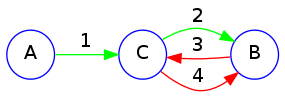
\includegraphics[width=\linewidth,keepaspectratio=true]{broadcast_loop.png}
  \caption{\emph{Broadcast Loops}: Edges are labeled in order of message transmission.  After receiving message 2, node B forwards it back to C as message 3, who will then forward it back to B as message 4 and so on...}
  \label{broadcast_loop}
\end{figure}

Each message, including the originals, will include the ID of the vehicles that witnessed (and participated in) the crash as well as the location of the event in order to facilitate authenticating the information and avoiding the scene, respectively.
Because each vehicle that witnesses the crash begins disseminating messages, there could be a large number of duplicate messages detecting the same event that are treated as distinct for the purposes of forwarding.
This is where data aggregation improves the efficiency of the system.

\subsection{Aggregation}

Instead of allowing each original message to be disseminated separately, we decided to aggregate them together into a single message whenever possible.
This saves a lot of network overhead by greatly reducing the number of packets that must be transmitted to disseminate the same information.
When a node receives more than one message that pertains to the same crash (as identified by the victim ID), the IDs of the witnesses are combined together into a single packet before forwarding.
In this way, each packet contains a subset of IDs corresponding to nodes that witnessed or participated in the event.
When a node receives such a packet, it may learn more than one ID as compared to only learning one without any aggregation.

In the case of multiple rebroadcasts, nodes will continuously update the packet they are broadcasting during each interval.
Therefore, if a node learns of another witness, or learns the ID of any crash victim(s), the next packet broadcasted will include this information.
This does not mean that the counter of how many rebroadcasts should be sent is reset, however, as this could prolong the life of the message to a wasteful point.
In this manner, forwarded messages typically contain only one or a small number of IDs initially.
As the message propagates further, aggregation will take place and each message will tend to contain more information about the event.


\section{Simulation and Results}
In this section of the report we will describe the implementation of the proposed protocol and simulate it using NS3 [NS3\_Reference]. We used NS3 to simulate the proposed crash model and measure some performance parameters. A set of classes are integrated with NS3 to simulate the existence of a highway with several lanes and vehicles driving on it. The mobility model used in our experiment is the highway mobility model provided by NS3. Basically, vehicles are created and initiated to drive on the highway at a starting point and with some velocity constraints such as minimum and maximum allowed speed. The existed model was very basic where vehicles are mostly driving the same speed and on the same lane, which renders it unrealistic. We improved this model by adding some randomness of the vehicles speed limits and allow them to by pass each others by driving on different lanes.

We also add the existence of the crash event. We initialize the simulation with two additional parameters, the crash vehicle and the time of the crash. The first parameters specifies the ID of the vehicle that will crash at a time specified by the second parameter. When a crash happens, the specified vehicle will stop and start sending "being in crash" messages and the neighbor vehicles will start disseminating the event information to the rest of the network.

It is worth mentioning that at each time step of the simulation, we write the position of each vehicle and the messages transferred to log files so we can verify the correctness of the implementation. The vehicle positions log file is used to feed a Java-based tool to vitalize the highway with all the vehicles driving on it during the whole simulation time. The other one, the transferred messages log file, is used to verify the validity of the dissemination and aggregation techniques used in our proposed protocol. We were able to visualize that the predefined vehicle is really having a crash and all other vehicles are successfully by passing it.

\noindent
\begin{figure}[h]
\centering
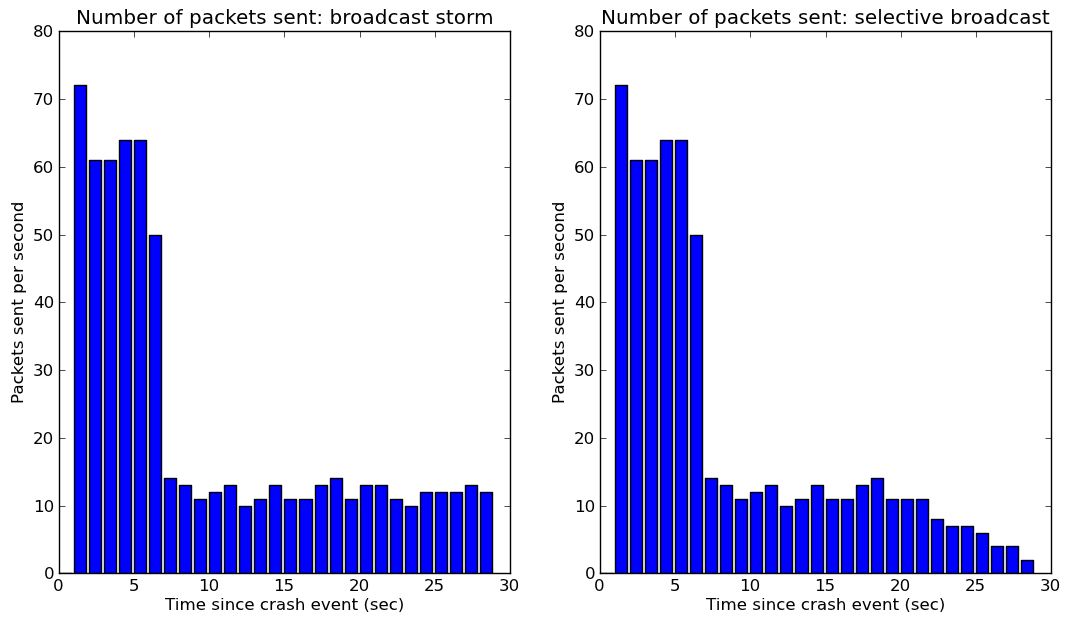
\includegraphics[scale=0.32]{Figure_01.png}
\caption{Broadcast storm versus selective broadcast}
\label{fig_storm_nostorm}
\end{figure}

Figure~\ref{fig_storm_nostorm} shows a comparison between the two cases of using broadcast storm and selective broadcast. We notice that in the case of using selective broadcast, the number of packets transferred in the network starts decreasing after 20 seconds of the simulation begins. The reason is because most vehicles have already received the crash message and start ignoring all message that are already received. On contrary, vehicles that use broadcast storm keeps on forwarding crash messages even if they already received the same messages before, this explains why after 20 seconds of the simulation begins, these vehicles keep on forwarding messages.

\noindent
\begin{figure}[h]
\centering
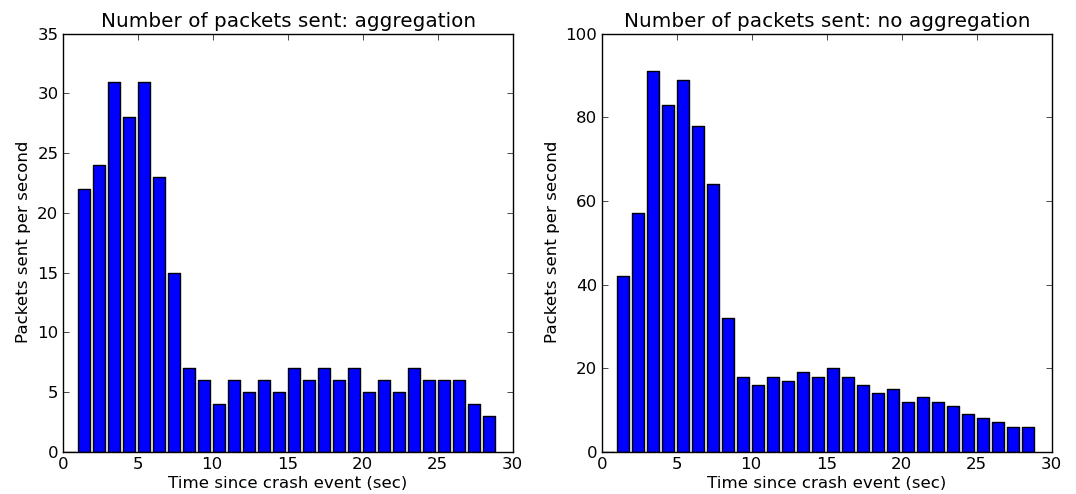
\includegraphics[scale=0.32]{Figure_02.png}
\caption{Aggregation versus non-aggregation}
\label{fig_aggregation_nonaggregation}
\end{figure}

Figure~\ref{fig_aggregation_nonaggregation} illustrate the case where vehicles use aggregation versus not using aggregation. It can be noticed that the number of messages sent when aggregation is not present is approximately three times more the number of messages sent when aggregation is used.

\noindent
\begin{figure}[h]
\centering
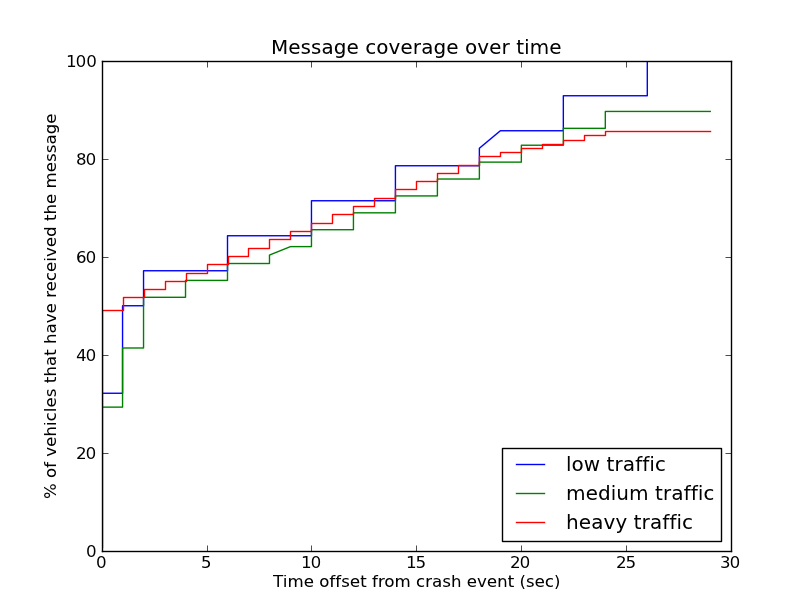
\includegraphics[scale=0.45]{Figure_03.png}
\caption{Message coverage over time}
\label{fig_msg_coverage}
\end{figure}

In Figure~\ref{fig_msg_coverage} we demonstrate the different dissemination patterns when low, medium and heavy traffic are present. It can be noticed that after roughly $25$ seconds of the simulation begins, all of the vehicle that are suppose to receive the crash message have already received it. At time $0$ second, or right after the simulation begins, we can notice that $50\%$ of the vehicles have received the crash message in heavy traffic case whereas only $30\%$ of them received the message in low and medium traffic. It is worth mentioning that the vehicles receiving the messages are the ones that are close to the crash area which means that the more the recipients are, the better the locality of the dissemination is. As time progressing, the message coverage curves for the three traffic density cases start the converge together. Moreover, it can be noticed that the case where heavy traffic exists have smoother message coverage curve due the presence or a lot of vehicles close to each others, thus vehicles carrying the message do not need to travel for some time to get into the vicinity of other vehicles to transfer the message to.




\section{Security Concerns}

In VANETs, the safety messages including traffic information messages (e.g. traffic condition), general safety-related messages (e.g. collision avoidance) and liability-related messages (e.g.when accidents happen) are critical to the security of drivers, their physical safety, and law enforcement. Therefore, VANET’s security should be considered at the design phase, rather than ad-hoc fixes after deployment. In the next paragraphs, we will describe different types of attacks on VANETs \cite{SecurityVANET, SecurityWSN} and security requirements to prevent such attacks.

\subsection{Attacks on VANET}

In this section, we will describe different attacks on VANETs. The attacks are classified according to the following criteria:
\begin{itemize}
\item Membership: Insider(I)/Outsider(O)
\item Motivation: Malicious(M)/Rational(R)
\item Method: Active(A)/Passive(P)
\item Scope: Local(L)/Extended(E)
\end{itemize}
For each attack we will use the following notation: Membership.Motivation.Method.Scope, e.g., I.M.A.L. means that the adversary is an insider, behaves maliciously and mounts an active attack in a local area.

\begin{itemize}
\item \emph{Jamming attack:} In this attack, the adversary wants to interfere with radio transmission. One simple jamming attack is the adversary continuously sends radio signal on a valid channel, thus preventing the legitimate vehicle from sending the radio signal. This is O.M.A.L.
\item \emph{Hidden vehicle:} This attack works as follows: whenever a vehicle broadcasts a warning message, the adversary will pretend to be in a better position to broadcast the message. Thus the message originator would stop broadcasting message to save traffic. The adversary in turn doesn’t broadcast the warning message further. Basically, the origin of the warning message is hidden by the adversary. This is O.M.A.L attack.
\item \emph{Tunnel attack:} This attack exploits the fact the GPS is disabled when the vehicle is going through the tunnel. The adversary can send fake information of GPS to the vehicle when it leaves the tunnel. This attack works as GPS is not authenticated. This is O.M.A.L attack.
\item \emph{Wormhole attack:} This is a collusion attack when we have 2 vehicles far apart but have a fast communication channel. The message from one vehicle is tunneled to another remote vehicle then the remote vehicle broadcasts the message. This way, an authenticated message is broadcast to another location. Essentially, there is a wormhole between 2 vehicles which helps broadcast a message to another location far apart. This is an I.M.A.E attack.
\item \emph{Bush telegraph attack:} This attack exploits the fact that if in every step there is a small error then in the end, the result would be totally different. The idea is if the error in each step is small, i.e., within the tolerance threshold then the neighbor would accept it. To implement this attack, the adversary needs to compromise a set of vehicles. This is I.M.A.L attack.
\item \emph{Sybil attack:} In this attack, a compromised vehicle claims multiple fake identities. This way, he can create fake positions, attract all the messages to him, etc. This is I.M.A.L.
\end{itemize}

\subsection{Security requirements for VANET}

To prevent the attacks described above, the following security requirements are needed:
\begin{itemize}
\item \emph{Authentication:} The sender identity must be authenticated as well as the sent messages.
\item \emph{Message Integrity:} There must be a mechanism to prevent(or detect) message’s integrity, i.e., detect the change of message by unauthorized vehicle.
\item \emph{Availability:} VANET must have the capability to prevent denial-of-service attack.
\item \emph{Non-repudiation:} The sender can not deny the message that he sent.This is really important in case of accidents, i.e., the vehicle that causes the accidents can not deny its responsibility.
\item \emph{Privacy:} This is really important as the drivers do not want the companies or govenment to trace all of his sent messages or locations.
\end{itemize}
Designing VANET to satisfy all the described security requirement is not a simple task. However, the fundamental step toward the security of VANET is to have a secure tamper resistant hardware to authenticate the vehicle and to sign the message by private key. Due to space constraints, we will not go into detailed solutions for all the listed security attacks. Instead, we will describe a solution for the authenticating disseminated data which is relevant to our project.

Itani et al. proposed in \cite{slow}, a Secure Bundle protocol, Sec-Bundle, to authenticate disseminated data sent through the networks. The proposed protocol is based on using an authentication structure, called a Bloom filter \cite{bloomF}. Such structure is used to verify the membership of a set of elements. In other words, using a Bloom filter, it is feasible to verify if a specific element belongs to a set or not. First, the source feeds all the data chunks in the Bloom filter, signs it with its private key using Identity-Based Encryption (IBE), and disseminates it. When an intermediate node, say a router, receives a data chunk, it compares it against the membership structure to see if it belongs to the set or not. If yes, the chunk is forwarded to the next hop, or dropped otherwise. Membership verification at intermediate nodes level is beneficial to drop bogus packets as soon as possible. The wireless link on which such packets are injected is the only link that carry them. The previous authenticated dissemination protocol can be used as a base infrastructure to address our problem.

\section{Conclusion}

Many of the known aggregation methods discussed rely on static topologies in order to guarantee convergence. These techniques also calculate very specific aggregation functions that do not necessarily apply to our environment. However, Flajolet-Martin sketch, hierarchical, and cluster based aggregation techniques may be applicable to our application.

Data dissemination in static networks is important when a node has content to send to several other nodes. CREW is one protocol in peer-to-peer networks. Habit is a proposed protocol that provides a solution for the dissemination problem in DTNs. Because VANETs are a special case of DTNs, techniques such as this can be applied in our problem domain. The study on dissemination in VANETs gave us important information on how the data should be forwarded to interested vehicles.  Our specific problem would probably merit using the bi-directional approach, however, because there is not as much information contained in a message identifying an event as there is in one identifying individual vehicles and so compression is not a concern.  Instead, the speed at which the data reaches each party is paramount.

Finally, we have to focus on security of VANETs as it will not only affect the information but also the health and life of driver. It also plays an important role in law enforcement, e.g., liability of accidents. The important characteristics of a VANET is it uses location information as a basic parameter, so it is not only vulnerable to general attacks on wireless sensor networks, such as jamming and sybil attacks, but it is also vulnerable to different types of position-based attacks such as wormhole and tunnel attacks. The basic step to solve all the security issues is to support authentication and having tamper resistant security hardware.  These are still open problems in this research domain and so we do not expect to address them in our current focus.

\bibliographystyle{IEEEtran}
\bibliography{project_report}
\end{document}
